\documentclass[10pt,a4paper]{article}
\usepackage[margin=2cm,headheight=26pt,headsep=10pt]{geometry}
\usepackage{times}
\usepackage{graphicx}
\usepackage[hidelinks]{hyperref}
% Page header required by the course on every page
\usepackage{fancyhdr}
\newcommand{\groupno}{XX}
\newcommand{\projname}{INN-RC: Lossless Image Steganography with Message-Conditioned Integer Coupling}
\fancypagestyle{uct}{%
  \fancyhf{}%
  \fancyhead[L]{\footnotesize UCT702 Research Project \quad Group No.: \groupno \\ Project Name: \projname}%
  \fancyhead[R]{\footnotesize Reetam Dutta (102318024)\\ Priyadarshi Vivekanand (102318048)}%
  \fancyfoot[C]{\footnotesize \thepage}%
  \renewcommand{\headrulewidth}{0.4pt}}

\pagestyle{uct}
\begin{document}
\thispagestyle{uct}
\section*{Supplementary material}
\subsection*{S1. Training curves}
\begin{center}
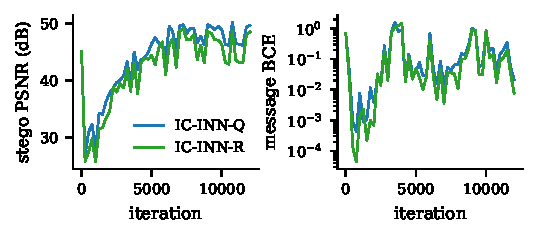
\includegraphics[width=0.75\textwidth]{../paper/figs/training.pdf}
\end{center}
Stego PSNR and message BCE of the training batches for both IC-INN models (12{,}000 iterations, CPU). For the first
10\% of the iterations only the message loss is active, so the network pushes a strong signal into the image and the
PSNR falls to about 25--30 dB. The image and overflow losses are then ramped in until 60\% of training and the PSNR
climbs to 46--49 dB while the message loss keeps going down. In the second half of training the uniform-noise
stand-in for rounding is replaced by real rounding with a straight-through gradient. The robustness-oriented model
(message weight 30) settles about 1.5 dB lower. The float-INN baseline log is in \texttt{models/finn\_s4\_train.txt};
its validation residual stayed at 42\% of pixels, which is why it never fits into PEE.

\subsection*{S2. How the numbers were produced}
All tables and plots in the paper are generated by \texttt{tools/make\_figures.py} directly from the CSV files written
by the MATLAB scripts:
\begin{itemize}
\item \texttt{run\_benchmark.m} -- lossless results for every test image, method and payload
(\texttt{results/bench\_a.csv}, \texttt{bench\_b.csv}, \texttt{bench\_c.csv});
\item \texttt{run\_attacks.m} -- message BER under noise and JPEG (\texttt{results/attacks.csv});
\item \texttt{run\_ablation\_aux.m} -- side-information size for the four coding choices;
\item \texttt{run\_baseline\_aux.m} -- side information the float-INN baseline would need.
\end{itemize}
Exact recovery is checked with \texttt{isequal} on the full image and message, not with a PSNR threshold. The same
seeds are used for every method, so all methods hide the same random message in the same image.

\subsection*{S3. Note on the TRK-07 baseline paper}
The link given for TRK-07 in the project guidelines opens ``Reversible data hiding in encrypted images using LWE-based
secret sharing'' (Scientific Reports, 2025), which does not use a neural network, and we could not find a paper with
the listed title. We therefore used DRRW (arXiv:2503.02490) and CRMark (ICCV 2025) as the reference work, and a
HiNet-style float invertible network with the same residual compensation as the implemented baseline.
\end{document}
